\section{\large Introducción}
En Colombia, la gestión de fotocomparendos ha sido objeto de controversia debido a fallas en la transparencia y posibles manipulaciones en el proceso de registro y validación de infracciones. La falta de un sistema confiable ha generado desconfianza entre los ciudadanos, lo que evidencia la necesidad de una solución que garantice la integridad, inmutabilidad y verificabilidad de la información.

La tecnología Blockchain ha demostrado ser una alternativa eficaz para el almacenamiento seguro y descentralizado de datos, asegurando que una vez registrados, estos no puedan ser alterados sin dejar rastro. A través de contratos inteligentes, es posible automatizar la validación y el procesamiento de fotocomparendos, reduciendo la intervención humana y minimizando el riesgo de corrupción o errores administrativos.

Este trabajo propone el diseño e implementación de un prototipo basado en Blockchain para la gestión de fotocomparendos en Bogotá, con el objetivo de garantizar la transparencia del proceso. Se utilizarán contratos inteligentes para registrar cada infracción, permitiendo que cualquier actor autorizado pueda verificar su autenticidad sin necesidad de intermediarios. Mediante pruebas y simulaciones, se evaluará la viabilidad del sistema, demostrando cómo esta tecnología puede fortalecer la confianza en los procesos de control de tránsito y mejorar la eficiencia en la gestión de sanciones.

\subsection{Formulación del problema}
La gestión de comparendos en Bogotá es un proceso de gran escala. Según datos del Observatorio de Movilidad, entre enero de 2018 y agosto de 2024 se emitieron más de 1.9 millones de comparendos a través de cámaras salvavidas, evidenciando la importancia sistémica de este proceso para la regulación del tránsito en la ciudad, como se presenta en la Figura~\ref{fig:estadisticas_comparendos} se observa los diferentes métodos utilizados para crear los comparendos. Esta operación se apoya en el sistema FÉNIX, una aplicación con infraestructura en la nube, cuya arquitectura de datos y control de acceso opera bajo un paradigma centralizado.

\begin{figure}[htbp]
    \begin{flushleft}
        \textbf{Figura 1}\\[2em]
        \textit{Estadísticas de comparendos emitidos en Bogotá entre enero de 2018 y agosto de 2024}
    \end{flushleft}
    \vspace{1em}
    \addcontentsline{lof}{figure}{Figura 1. Estadísticas de comparendos emitidos en Bogotá entre enero de 2018 y agosto de 2024}
    \centering
    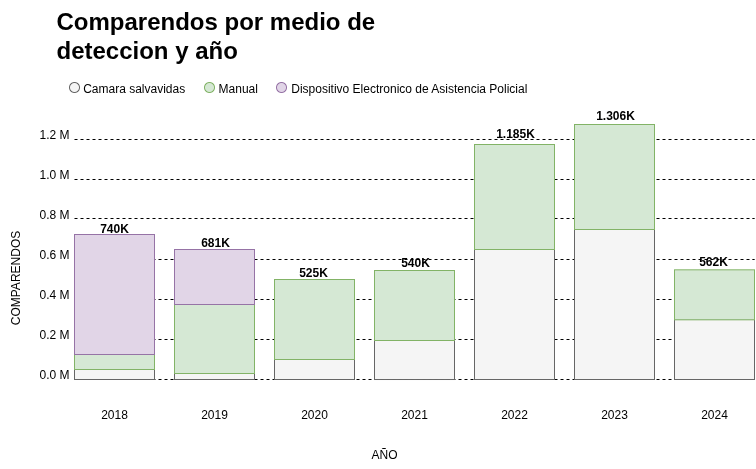
\includegraphics[width=0.8\textwidth]{Images/numComparendos.png}
    \vspace{2em}
    \begin{flushleft}
        \textit{Nota.} Elaboración propia basado en datos del Observatorio de Movilidad.
    \end{flushleft}
    \refstepcounter{figure}\label{fig:estadisticas_comparendos}
\end{figure}

En el sistema actual, la validez e inmutabilidad de los registros de infracciones se fundamenta en los procedimientos administrativos y en la gestión de los funcionarios responsables del sistema \parencite{C112_2018}. Los cambios en la información solo pueden ser detectados por las entidades autorizadas, lo que implica que el control sobre los registros depende directamente de la correcta aplicación de las políticas internas y del seguimiento realizado por dichas entidades \parencite{Sentencia123_2019}. La evidencia generada se conserva bajo un modelo centralizado, en el cual la confianza en la integridad de los datos se sostiene en mecanismos administrativos y controles internos, más que en garantías técnicas accesibles públicamente \parencite{DAFP_Lineamientos_2021}. La potestad sancionatoria y el debido procedimiento administrativo aseguran la validez de los actos administrativos y la correcta motivación en la imposición de sanciones (Corte Constitucional, 2022; Gamero Casado y Fernández Ramos, s.f.).

De acuerdo con la Auditoría de Cumplimiento de la Contraloría de Bogotá (2024), en el proceso de desarrollo del sistema FÉNIX se identificaron dificultades relacionadas con la supervisión contractual, lo que derivó en retrasos, duplicidad de sistemas y un presunto detrimento patrimonial estimado en más de \$8.000 millones de pesos. Estos hallazgos reflejan que, desde su implementación, la plataforma ha enfrentado retos significativos en materia de gobernanza y gestión, los cuales han tenido impacto en la eficiencia administrativa y en la sostenibilidad financiera del proyecto.

Estas debilidades se manifiestan en la operación técnica actual. A nivel operativo, el riesgo de integridad se materializa en una fricción a gran escala con la ciudadanía. Un análisis correlacional de fuentes oficiales para el primer semestre de 2025 revela la magnitud de esta fricción: frente a 457.000 comparendos impuestos [Observatorio de Movilidad, 2025], se gestionaron 155.854 PQRSD [Informe de Gestión PQRSD, 2025]. De estos datos se deduce una Tasa de Impugnación general del 34.1\%, un indicador cuantitativo que sugiere que al menos uno de cada tres actos administrativos del sistema genera una disputa formal, reflejando una carga administrativa insostenible y un déficit de confianza.

La desconfianza generada por estas opacidades y dificultades procesales crea un vacío que es explotado por terceros, afectando directamente al ciudadano. Reportajes de prensa documentan cómo la ausencia de canales oficiales percibidos como confiables ha fomentado la aparición de redes de fraude, como el caso de Juzto.co, donde miles de ciudadanos fueron estafados con promesas de impugnaciones garantizadas, resultando en trámites inconclusos y mayores deudas \parencite{Semana_Juzto_2023}.

La identificación de estas limitaciones permite estructurar el problema en torno a variables que reflejan tanto el modelo de confianza actual como sus impactos técnicos, operativos y financieros. La Tabla~\ref{tab:comparacion_bd_blockchain} sintetiza estas variables y los indicadores asociados, mostrando cómo el paradigma centralizado de gestión condiciona la integridad de los datos, la eficiencia administrativa, la confianza ciudadana y la sostenibilidad del sistema.

\begin{table}[htbp]
    \begin{flushleft}
        \textbf{Tabla 1}\\[2em]
        \textit{Comparación entre bases de datos tradicionales y blockchain para gestión de registros gubernamentales}
    \end{flushleft}
    \vspace{1em}
    \addcontentsline{lot}{table}{Tabla 1. Comparación entre bases de datos tradicionales y blockchain para gestión de registros gubernamentales}
    \centering
    \begin{tabular}{p{4.5cm} p{5.2cm} p{5.2cm}}
        \toprule
        \textbf{Característica} & \textbf{Base de Datos Convencional} & \textbf{Blockchain} \\
        \midrule
        Modelo de confianza & Se basa en un administrador central (entidad de TI) & Confianza distribuida entre múltiples nodos \\
        Inmutabilidad & Registros pueden ser modificados o eliminados por administradores & Los registros son inmutables por diseño \\
        Trazabilidad / Auditoría & Depende de la implementación y control interno & Historial completo e inalterable disponible \\
        Riesgo de corrupción interna & Alto, si hay privilegios indebidos o colusión & Bajo, no se puede alterar sin consenso de la red \\
        Seguridad criptográfica & Opcional, no siempre integrada nativamente & Integrada (firmas digitales, hashes, cifrado) \\
        Disponibilidad / tolerancia a fallos & Riesgo de puntos únicos de falla & Alta disponibilidad por replicación descentralizada \\
        Velocidad de operación & Alta velocidad en lectura/escritura & Menor velocidad, prioriza integridad y consenso \\
        \bottomrule
    \end{tabular}
    \vspace{2em}
    \begin{flushleft}
        \textit{Nota.} Elaboración propia.
    \end{flushleft}
    \refstepcounter{table}\label{tab:comparacion_bd_blockchain}
\end{table}

En síntesis, el problema se formula como un Riesgo de Integridad de Datos inherente al paradigma de confianza centralizada del sistema de fotocomparendos. Este riesgo se encuentra documentado por debilidades fundacionales en la gobernanza del proyecto y se manifiesta en consecuencias medibles: (i) una Tasa de Impugnación del 34.1\%; (ii) una carga operativa superior a 155 mil PQRSD semestrales; (iii) un presunto detrimento patrimonial por más de \$8.000 millones; y (iv) la vulnerabilidad de la ciudadanía a esquemas fraudulentos derivados de la falta de transparencia institucional.

Ante este panorama, surge la necesidad de explorar arquitecturas que permitan sustituir la confianza administrativa por garantías criptográficas. La pregunta central que guía este trabajo es:

\textbf{¿Cómo mitigar el Riesgo de Integridad de Datos en el proceso de fotocomparendos en Bogotá?} 

\subsection{Objetivos}
\paragraph{Objetivo General}
Desarrollar un prototipo para apoyar el registro y trazabilidad de estados en el proceso de fotocomparendos en Bogotá, aplicando tecnologías de redes distribuidas, con el fin de fortalecer la integridad, la autenticidad de la información, y reducir los riesgos asociados a su confidencialidad.

\paragraph{Objetivos específicos}
\begin{itemize}
    \item Analizar el proceso actual de registro de fotocomparendos en Bogotá, a partir del marco jurídico y regulatorio que lo rige y de los informes de auditoría emitidos por la secretaria distrital de movilidad sobre la gestión de comparendos, para identificar requisitos funcionales, no funcionales y vulnerabilidades que el prototipo debe proporcionar.
    \item Desarrollar un prototipo con arquitectura híbrida fundamentada en la técnica de descomposición por confianza, integrando tecnologías de almacenamiento distribuido y contenido cifrado, asegurando que cada transacción incorpore los metadatos del comparendo y disponiendo de una interfaz básica para demostrar que es posible un aplicativo transparente y confiable.
    \item Evaluar la viabilidad del prototipo desarrollado, mediante la ejecución de un plan de pruebas funcionales y evaluación de métricas de desempeño en un entorno de pruebas, para validar las condiciones de inmutabilidad, trazabilidad y seguridad.
\end{itemize}

\subsection{Impacto o alcance esperado}
\paragraph{Alcance}
\textbf{Enfoque y delimitación geográfica:} Este trabajo se circunscribe al proceso de trazabilidad de estados de multas de tránsito automatizadas (fotomultas) emitidas por la Secretaría Distrital de Movilidad de Bogotá. Se excluyen de manera explícita los siguientes aspectos:
\begin{itemize}
    \item Multas impuestas de forma presencial por agentes de tránsito.
    \item Procesos sancionatorios de otras ciudades o entidades territoriales.
    \item Funcionalidades de recaudo y pasarelas de pago (solo se registra el estado del pago, no se procesa el pago en sí).
\end{itemize}

\textbf{Componentes del prototipo:} El prototipo aborda los siguientes módulos funcionales:
\begin{itemize}
    \item \textbf{Registro inmutable de la infracción:} Captura de metadatos (placa, fecha, hora, ubicación y tipo de infracción) y publicación del identificador de la evidencia en la blockchain (Hyperledger Fabric).
    \item \textbf{Almacenamiento descentralizado de evidencias:} Carga de la imagen o video de la fotomulta en IPFS y obtención de su hash.
    \item \textbf{Verificación pública:} Servicio de consulta que permite contrastar el hash guardado en la cadena con el archivo almacenado en IPFS.
    \item \textbf{Gestión del ciclo de vida de la multa:} Estados: Generada → Notificada → En apelación → Pagada → Cerrada. Cada transición queda registrada mediante eventos de contrato inteligente.
    \item \textbf{Interfaz mínima:} Panel Web para: (i) agentes que registran la infracción y (ii) ciudadanos que consultan la autenticidad y el estado de su fotomulta.
\end{itemize}

\textbf{Fuera del alcance:}
\begin{itemize}
    \item Integración completa con sistemas legados del RUNT o SIMIT; se simula mediante datos de prueba.
    \item Implementación de un modelo económico (tarifas de gas, costos operativos reales).
    \item Implementación de algoritmos de detección automática de infracciones (visión por computador). Se parte de que la cámara ya detectó la infracción y generó la evidencia.
    \item Despliegue en un entorno de producción o capacidad más de 10 usuarios.
\end{itemize}

\textbf{Entregables:}
\begin{itemize}
    \item Contrato inteligente en Solidity (o «chaincode» en Go, según la red seleccionada) con pruebas unitarias.
    \item Script de despliegue de red Hyperledger Fabric e instalación de IPFS local.
    \item Aplicación Web de demostración (frontend ligero) conectada a los servicios anteriores.
    \item Manual técnico que documenta la arquitectura y el flujo de datos.
    \item Informe de resultados de las pruebas funcionales y de rendimiento básico.
\end{itemize}

\textbf{Criterios de éxito:}
\begin{itemize}
    \item Tiempo medio de publicación de una infracción $\leq$ 3 s en entorno de laboratorio.
    \item Coincidencia 100\% entre el hash almacenado en la cadena y la evidencia recuperada desde IPFS.
    \item Trazabilidad completa del historial de estados para al menos 50 multas de prueba.
    \item Ausencia de fallos críticos en pruebas de carga con 10 transacciones concurrentes.
\end{itemize}

\paragraph{Limitaciones del Prototipo}
Es fundamental reconocer que, como prototipo desarrollado en un contexto académico, el presente estudio presenta ciertas limitaciones que definen el alcance de sus conclusiones y delinean claras oportunidades para futuras investigaciones. Las principales limitaciones son:

\textbf{Entorno de Validación:}
\begin{itemize}
    \item \textbf{Validación en Entorno de Laboratorio:} El prototipo fue diseñado, desplegado y evaluado en un entorno de simulación controlado. No se sometió a pruebas en una infraestructura productiva real con la carga de transacciones y el volumen de usuarios que gestiona actualmente la Secretaría de Movilidad.
    \item \textbf{Uso de Datos Simulados:} Debido a estrictas normativas de privacidad y protección de datos personales que impiden el acceso a información real de ciudadanos y vehículos, todas las pruebas se realizaron con datos sintéticos.
    \item \textbf{Suposiciones sobre la Calidad de la Evidencia:} El sistema asume que las evidencias fotográficas (imágenes de fotocomparendos) son capturadas con una calidad suficiente para su procesamiento.
\end{itemize}

\textbf{Integración y Comparación con Sistemas Existentes:}
\begin{itemize}
    \item \textbf{Integración Simulada con Sistemas Externos:} La interacción con plataformas gubernamentales clave como el RUNT y el SIMIT fue simulada a través de APIs de prueba (mocks).
    \item \textbf{Ausencia de Benchmarking Directo con el Sistema Actual (Fénix):} La falta de acceso al código fuente y a la arquitectura interna del sistema Fénix impidió realizar una comparación cuantitativa y directa.
\end{itemize}

\textbf{Aspectos Técnicos y de Escalabilidad:}
\begin{itemize}
    \item \textbf{Proyección de Costos como Escenario de Referencia:} Los costos de infraestructura y desarrollo estimados corresponden a un escenario de referencia.
    \item \textbf{Estrategia de Persistencia en IPFS:} Para que la evidencia digital permanezca disponible a largo plazo en IPFS, es necesario que al menos un nodo la mantenga "pineada".
\end{itemize}

\textbf{Seguridad y Robustez:}
\begin{itemize}
    \item \textbf{Ausencia de Pruebas de Seguridad Ofensivas:} El alcance del proyecto no incluyó la realización de auditorías de seguridad formales sobre los contratos inteligentes ni pruebas de penetración sobre la aplicación web.
\end{itemize} 